\documentclass[12pt, a4paper, twoside, romanian]{teza-upb}
\setcounter{secnumdepth}{3}
\setcounter{tocdepth}{3}
 
% --- Encoding și fonturi (OBLIGATORIU pentru diacritice cu pdflatex) ---
\usepackage[T1]{fontenc}      % codare corectă a fontului pentru ă, î, â, ș, ț
\usepackage{lmodern}          % font vectorial care suportă bine T1
 
% NOTĂ: am scos opțiunea [demo] de la graphicx — aceea înlocuia toate
% imaginile cu dreptunghiuri goale. La varianta finală cu figuri reale
% folosește graphicx fără opțiuni.
\usepackage{graphicx}
\usepackage[top=2cm, bottom=2cm, left=2cm, right=2cm, headsep=1cm, footskip=1cm]{geometry}
\usepackage[romanian]{babel}
\usepackage{ragged2e}
\usepackage{color}
\usepackage{pdfpages}
\usepackage[bookmarks, bookmarksopen=true, pdftitle={Lucrare de licenta - ETTIway}, linktocpage]{hyperref}
\usepackage{listings}
\usepackage{float}
\usepackage{amsmath}
\usepackage{amssymb}
\usepackage{tabularx}
\usepackage{booktabs}
\usepackage{longtable}
\linespread{1.3}
\AtBeginDocument{\justifying}
 
\definecolor{codegreen}{rgb}{0,0.6,0}
\definecolor{codegray}{rgb}{0.5,0.5,0.5}
\definecolor{codepurple}{rgb}{0.58,0,0.82}
\definecolor{backcolour}{rgb}{0.95,0.95,0.92}
 
\lstdefinestyle{mystyle}{
    backgroundcolor=\color{backcolour},
    commentstyle=\color{codegreen},
    keywordstyle=\color{blue},
    numberstyle=\tiny\color{codegray},
    stringstyle=\color{codepurple},
    basicstyle=\ttfamily\footnotesize,
    breakatwhitespace=false,
    breaklines=true,
    captionpos=b,
    keepspaces=true,
    numbers=left,
    numbersep=5pt,
    showspaces=false,
    showstringspaces=false,
    showtabs=false,
    tabsize=2
}
\lstset{style=mystyle}
 
\begin{document}
 
\author{Fraticiu Vlad-Alexandru}
\title{ETTIway - Sistem de Navigare Interactivă Campus}
\facultatea{Facultatea de Electronică, Telecomunicații și Tehnologia Informației}
\tiplucrare{licență}
\domeniu{Electronică, Telecomunicații și Tehnologia Informației}
\catedra{Telecomunicații}
\campus{Leu}
\program{Rețele și Software de Telecomunicații}
\titlulobtinut{Inginer}
\director{ș.l. dr. ing. Laurențiu BOICESCU}
\submissionmonth{Iunie}
\submissionyear{2026}
 
\pagenumbering{roman}
\pagestyle{empty}
\titlep
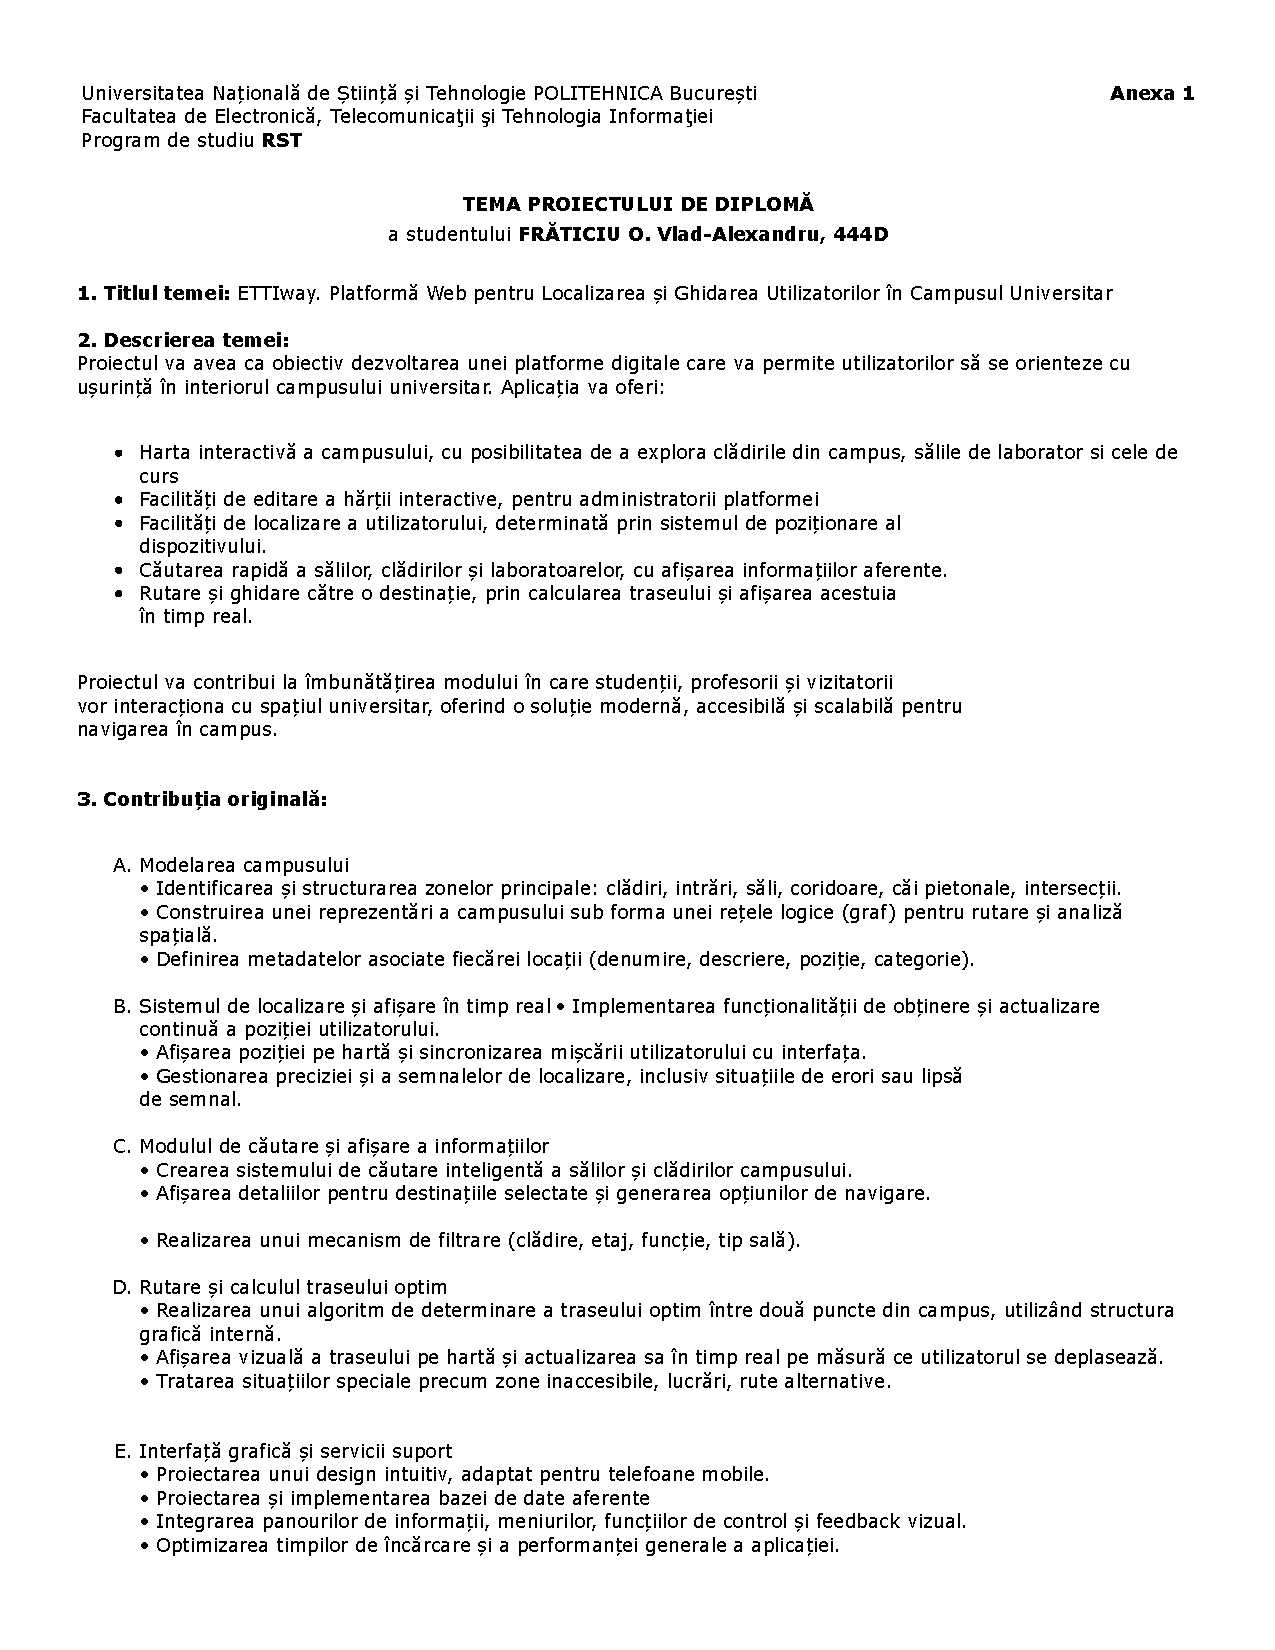
\includepdf[pages={1,2}]{Anexa1.2.pdf}
\declaratiep
\tableofcontents
\pagestyle{plain}
 
\abbreviations{
    API = Application Programming Interface \\
    OSM = OpenStreetMap \\
    GPS = Global Positioning System \\
    REST = Representational State Transfer \\
    JSON = JavaScript Object Notation \\
    HTTP = Hypertext Transfer Protocol \\
    JPA = Java Persistence API \\
    WKB = Well-Known Binary \\
    WKT = Well-Known Text \\
    SRS = Spatial Reference System
}
 
\afterpreface
\pagestyle{plain}
 
\chapter*{Introducere}
\addcontentsline{toc}{chapter}{Introducere}
\section{Contextul Proiectului}
Problema principală care apare frecvent într-un campus universitar este de a integra navigația exterioară cu cea interioară în corpuri, săli și laboratoare, într-un singur flux digital coerent. Plecând de la această problemă, lucrarea propune ETTIway, o platformă construită pentru a aduce la un loc navigarea exterioară cât și pe cea interioară într-o experiență unitară atât pentru studenți, cât și pentru personalul universitar. Obiectivul principal a fost dezvoltarea unei soluții capabile să ofere localizare contextuală, căutare rapidă a punctelor de interes și suport pentru rutare între locații relevante din campus.
 
Arhitectura tehnică îmbină un backend realizat cu Spring Boot, responsabil de expunerea serviciilor și gestionarea datelor, cu o interfață web interactivă construită cu JavaScript și Leaflet, orientată spre claritate vizuală și timp de răspuns redus. O contribuție practică importantă este integrarea stratului de date spațiale provenit din OpenStreetMap, care permite reprezentarea fidelă a infrastructurii campusului și extinderea facilă către noi zone. În completarea funcțiilor de bază, platforma include mecanisme de afișare contextuală a informațiilor despre clădiri și spații, precum și o bază pentru rutare inteligentă între puncte selectate. Din perspectiva operațională, soluția oferă și suport pentru administrarea datelor geografice, astfel încât actualizarea hărților, a denumirilor și a punctelor de interes să poată fi realizată rapid, cu impact minim asupra utilizatorului final.
 
\section{Motivația și Obiectivele}
Motivația principală a proiectului pornește din dificultățile reale întâlnite în orientarea zilnică din campus: identificarea rapidă a clădirilor, localizarea corectă a sălilor și parcurgerea eficientă a traseelor dintre puncte relevante. În absența unei soluții unificate, utilizatorii sunt nevoiți să combine surse multiple de informație, adesea incomplete sau necorelate între ele. Din această perspectivă, ETTIway urmărește să ofere o experiență digitală coerentă, care să reducă timpul de căutare și să îmbunătățească orientarea atât pentru utilizatorii noi, cât și pentru cei familiarizați cu infrastructura universitară.
 
Obiectivele urmărite în dezvoltarea platformei au fost definite pe două direcții complementare: utilitatea practică pentru utilizatorul final și mentenabilitatea tehnică a sistemului. Astfel, platforma a fost proiectată pentru a integra harta campusului cu date indoor/outdoor într-o interfață unitară, pentru a permite căutarea contextuală a punctelor de interes și pentru a susține rutarea între locații relevante. În paralel, arhitectura aplicației a fost gândită astfel încât actualizarea datelor geografice și extinderea către noi clădiri sau zone să poată fi realizate rapid, fără modificări majore în fluxul de utilizare.
 
\section{Metodologia și contribuția proprie}
Metodologia de dezvoltare a fost structurată în etape succesive, astfel încât fiecare componentă a sistemului să poată fi validată înainte de integrarea finală. În prima etapă a fost realizată analiza cerințelor funcționale și nefuncționale, cu accent pe scenariile reale de utilizare: localizarea rapidă a unei clădiri, identificarea unei săli și parcurgerea unui traseu relevant în campus. Pe baza acestei analize a fost definită arhitectura aplicației, separată pe nivelul de prezentare (frontend), nivelul serviciilor (backend) și nivelul datelor geografice. Implementarea a fost realizată incremental, prin dezvoltarea și testarea separată a modulelor de vizualizare, căutare și gestiune a datelor indoor, urmată de integrarea lor într-un flux unitar.
 
Contribuția proprie vizează atât partea tehnică, cât și partea de organizare a datelor spațiale. La nivel de date, contribuția include structurarea seturilor geospațiale utilizate de aplicație, adaptarea lor pentru scenariile de navigare și construirea unei baze extensibile pentru adăugarea de noi clădiri, niveluri și elemente de infrastructură. Rezultatul este o soluție funcțională, ușor de extins, orientată spre utilizare practică în mediul universitar.
\chapter{Fundamente teoretice și tehnologii utilizate}
\label{cap:fundamente}
 
Acest capitol prezintă fundamentul teoretic și tehnologic pe care se sprijină
platforma ETTIway. Sunt abordate, în mod gradual, conceptele de bază ale
sistemelor de navigare digitală, particularitățile navigării în spații
exterioare și interioare, modul de reprezentare a datelor geospațiale, precum
și tehnologiile concrete folosite în implementare. Scopul acestui capitol este
de a oferi cititorului contextul necesar pentru a înțelege deciziile de
proiectare descrise în capitolele următoare, plecând de la principiile generale
și ajungând la instrumentele specifice care au stat la baza dezvoltării
aplicației.
 
\section{Sisteme de navigare și hărți digitale}
\label{sec:sisteme-navigare}
 
Un sistem de navigare digitală reprezintă un ansamblu de componente software și
de date care permite unui utilizator să se localizeze într-un spațiu, să
identifice puncte de interes și să determine trasee între acestea. Spre
deosebire de hărțile tipărite, hărțile digitale sunt interactive: utilizatorul
poate mări sau micșora nivelul de detaliu, poate filtra informația afișată și
poate interoga elementele de pe hartă pentru a obține date suplimentare. Această
interactivitate este esențială într-un mediu complex, cum este un campus
universitar, unde densitatea informației relevante este ridicată, iar nevoile
utilizatorilor variază considerabil de la o situație la alta.
 
În general, un sistem de navigare modern se construiește pe trei piloni
fundamentali: un strat de date geografice care descrie spațiul fizic, un motor
de procesare care interpretează aceste date și răspunde interogărilor, și o
interfață de vizualizare care prezintă informația într-o formă accesibilă
utilizatorului. Calitatea experienței finale depinde de modul în care aceste
trei niveluri sunt corelate și optimizate. Un strat de date incomplet conduce
la rezultate inexacte, un motor de procesare lent degradează experiența
interactivă, iar o interfață confuză anulează beneficiile unei baze de date
bine structurate.
 
Hărțile digitale interactive au cunoscut o dezvoltare accentuată odată cu
apariția bibliotecilor de cartografie web, care permit afișarea hărților direct
în browser, fără instalarea unor aplicații dedicate. Acest model, în care harta
este servită ca o aplicație web, prezintă avantaje semnificative din punct de
vedere al accesibilității: utilizatorul are nevoie doar de un browser modern și
de o conexiune la internet, fără dependențe de sistem de operare sau de hardware
specializat. ETTIway adoptă tocmai acest model, fiind o aplicație web ce poate
fi accesată de pe orice dispozitiv cu un browser compatibil.
 
\subsection{Reprezentarea hărților prin dale (tiles)}
\label{subsec:tiles}
 
Una dintre tehnicile fundamentale folosite în cartografia web este împărțirea
hărții în dale (în engleză \textit{tiles}), imagini pătrate de dimensiune fixă,
de regulă 256 pe 256 de pixeli, care acoperă o anumită zonă geografică la un
anumit nivel de zoom. În loc să se încarce o singură imagine de dimensiune
foarte mare, harta este compusă dinamic din mai multe asemenea dale, dintre care
se afișează doar cele vizibile în fereastra curentă. Pe măsură ce utilizatorul
se deplasează sau modifică nivelul de zoom, sunt încărcate noile dale necesare,
iar cele care ies din câmpul vizual sunt eliberate din memorie.
 
Acest mecanism de afișare are mai multe avantaje practice. În primul rând,
reduce volumul de date transferat la un moment dat, deoarece se transmit doar
porțiunile vizibile ale hărții. În al doilea rând, permite stocarea în memoria
cache a dalelor deja descărcate, ceea ce accelerează navigarea repetată prin
aceeași zonă. În al treilea rând, sistemul de dale se pretează foarte bine la
mai multe niveluri de detaliu: la niveluri mici de zoom se afișează contururi
generale, iar la niveluri mari apar detalii fine, precum clădiri individuale,
intrări sau trasee pietonale. Această organizare piramidală a datelor este
folosită de majoritatea serviciilor de hărți web și constituie fundamentul pe
care se construiește și experiența vizuală din ETTIway.
 
\section{Navigarea exterioară și navigarea interioară}
\label{sec:exterior-interior}
 
O distincție esențială în domeniul navigării este cea dintre navigarea
exterioară (\textit{outdoor}) și cea interioară (\textit{indoor}). Cele două
tipuri de navigare ridică probleme diferite atât din punct de vedere al
achiziției datelor, cât și din punct de vedere al reprezentării și al modului de
interacțiune cu utilizatorul. Una dintre contribuțiile centrale ale lucrării de
față este tocmai integrarea acestor două dimensiuni într-un flux unitar, astfel
încât utilizatorul să poată trece în mod natural de la nivelul campusului la
nivelul unei clădiri și, mai departe, la nivelul unei săli sau al unui laborator.
 
\subsection{Navigarea exterioară}
\label{subsec:outdoor}
 
Navigarea exterioară se referă la orientarea în spațiul deschis: identificarea
clădirilor, a aleilor, a intrărilor și a traseelor dintre diferite puncte de
interes ale campusului. La acest nivel, datele geografice sunt în general
disponibile prin servicii cartografice publice și pot fi reprezentate în
sisteme de coordonate geografice standard, exprimate prin latitudine și
longitudine. Pozițiile sunt asociate unui sistem global de referință, ceea ce
permite suprapunerea corectă a diferitelor straturi de informație și
compatibilitatea cu datele provenite din surse externe.
 
Pentru un campus universitar, navigarea exterioară presupune reprezentarea
fidelă a infrastructurii: conturul clădirilor, denumirile acestora, aleile
pietonale, drumurile de acces și punctele de interes precum intrările
principale, bibliotecile, cantinele sau punctele de orientare. Provocarea
principală la acest nivel nu este atât tehnologică, cât legată de completitudinea
și acuratețea datelor: o hartă exterioară este utilă doar în măsura în care
reflectă corect realitatea din teren și este actualizată atunci când
infrastructura se modifică.
 
\subsection{Navigarea interioară}
\label{subsec:indoor}
 
Navigarea interioară se ocupă de orientarea în interiorul clădirilor:
identificarea sălilor, a laboratoarelor, a etajelor și a traseelor dintre
acestea. Acest tip de navigare ridică dificultăți suplimentare în comparație cu
cea exterioară. Pe de o parte, datele de interior nu sunt, în general,
disponibile în servicii cartografice publice și trebuie construite manual,
plecând de la planuri ale clădirilor. Pe de altă parte, reprezentarea spațiului
interior implică o componentă verticală — etajele — care nu poate fi exprimată
printr-o simplă pereche de coordonate plane, ci necesită un mecanism de
organizare pe niveluri.
 
În cadrul ETTIway, navigarea interioară este tratată prin asocierea fiecărei
clădiri cu un set de planuri de etaj, fiecare plan corespunzând unui nivel
distinct al clădirii. Utilizatorul poate selecta o clădire de pe harta
exterioară și poate apoi naviga între etajele acesteia, vizualizând dispunerea
sălilor și a spațiilor relevante. Această abordare, în care nivelul exterior și
cel interior sunt corelate prin intermediul entității „clădire”, permite o
tranziție coerentă între cele două perspective și constituie nucleul
funcțional al platformei.
 
\subsection{Integrarea celor două niveluri}
\label{subsec:integrare}
 
Marea provocare a unui sistem complet de navigare în campus este unificarea
celor două niveluri într-o singură experiență, fără discontinuități. În multe
soluții existente, navigarea exterioară și cea interioară sunt tratate de
aplicații separate sau de surse de date necorelate, ceea ce obligă utilizatorul
să combine manual informații provenite din mai multe locuri. ETTIway propune o
abordare integrată, în care o clădire selectată pe harta exterioară devine
punctul de intrare către reprezentarea interioară a acesteia, păstrând astfel un
fir narativ continuu pentru utilizator. Această integrare reprezintă una dintre
contribuțiile practice principale ale lucrării și este detaliată în capitolele
dedicate arhitecturii și implementării.
 
\section{Date geospațiale și modelarea informației geografice}
\label{sec:date-geospatiale}
 
Fundamentul oricărui sistem de navigare îl constituie datele geospațiale, adică
informația care descrie poziția și forma obiectelor în spațiu. Modul în care
aceste date sunt structurate, stocate și interogate influențează direct
performanța și flexibilitatea întregului sistem. În această secțiune sunt
prezentate conceptele de bază necesare înțelegerii stratului de date al
aplicației ETTIway.
 
\subsection{Sisteme de coordonate și sisteme de referință spațială}
\label{subsec:srs}
 
Pentru a putea localiza un obiect pe suprafața Pământului este necesar un sistem
de referință spațială (SRS), care definește modul în care coordonatele numerice
se traduc în poziții reale. Cel mai răspândit sistem de referință folosit în
aplicațiile web este cel bazat pe latitudine și longitudine, exprimate în grade,
asociat unui model standardizat al Pământului. Acest sistem este utilizat pe
scară largă deoarece este compatibil cu majoritatea surselor de date publice și
cu serviciile de poziționare prin satelit.
 
Pe lângă sistemul geografic exprimat în grade, în cartografia web este frecvent
folosită și o proiecție plană, care transformă suprafața curbă a Pământului
într-un plan, facilitând afișarea hărților pe ecran. Trecerea între diferite
sisteme de referință se numește reproiecție și trebuie tratată cu atenție,
deoarece o suprapunere incorectă a straturilor de date conduce la afișarea
eronată a obiectelor. În cadrul ETTIway, consecvența sistemului de referință
între datele provenite din diverse surse este o condiție necesară pentru
alinierea corectă a infrastructurii campusului.
 
\subsection{Reprezentarea geometriilor: WKT și WKB}
\label{subsec:wkt-wkb}
 
Obiectele geografice — puncte, linii și poligoane — sunt descrise prin
geometrii. O clădire poate fi reprezentată ca un poligon, o alee ca o linie, iar
un punct de interes ca un singur punct. Pentru a stoca și a transmite aceste
geometrii există formate standardizate. Formatul textual WKT (\textit{Well-Known
Text}) descrie geometriile într-o formă lizibilă pentru om, în timp ce formatul
binar WKB (\textit{Well-Known Binary}) le codifică într-o reprezentare compactă,
optimizată pentru stocare și transfer. Ambele formate sunt larg acceptate de
bazele de date spațiale și de bibliotecile de procesare geografică, ceea ce
asigură interoperabilitatea între componentele sistemului.
 
Folosirea unor formate standardizate de reprezentare a geometriilor este
importantă pentru extensibilitatea aplicației: datele pot fi importate din surse
externe, prelucrate cu instrumente specializate și apoi consumate de aplicație,
fără a fi nevoie de conversii proprietare. Acest aspect susține unul dintre
obiectivele declarate ale proiectului, și anume capacitatea de a adăuga ușor noi
clădiri și zone fără modificări majore în logica aplicației.
 
\subsection{OpenStreetMap ca sursă de date}
\label{subsec:osm}
 
OpenStreetMap (OSM) este un proiect colaborativ care pune la dispoziție date
geografice deschise, contribuite și întreținute de o comunitate largă de
utilizatori din întreaga lume. Datele OSM acoperă o gamă variată de elemente:
drumuri, clădiri, alei pietonale, puncte de interes și multe altele. Faptul că
aceste date sunt deschise și pot fi descărcate și prelucrate liber le face o
sursă valoroasă pentru aplicațiile de navigare, mai ales în contextul în care
construirea de la zero a unui set complet de date geografice ar fi extrem de
costisitoare.
 
În cadrul ETTIway, datele provenite din OpenStreetMap sunt folosite pentru
reprezentarea infrastructurii exterioare a campusului, în special pentru
afișarea drumurilor și a aleilor. Modelul de date OSM organizează informația în
jurul a trei tipuri de elemente fundamentale: noduri, care reprezintă puncte
individuale definite prin coordonate; căi, care reprezintă secvențe ordonate de
noduri și pot descrie atât linii, cât și conturul unor suprafețe; și relații,
care grupează mai multe elemente pentru a descrie structuri complexe. Fiecărui
element i se pot asocia etichete sub formă de perechi cheie–valoare, care îi
descriu semnificația, de exemplu tipul de drum sau funcția unei clădiri.
Această structură flexibilă permite filtrarea și selectarea elementelor
relevante pentru navigarea în campus. Datele extrase din OpenStreetMap sunt
adaptate scenariilor de navigare din campus, fiind reținute doar elementele
relevante — drumuri, alei și contururi de clădiri — și eliminate informațiile
care nu prezintă interes pentru aplicație. Organizarea atentă a stratului de
date reprezintă, de altfel, o parte semnificativă a contribuției proprii
descrise în lucrare.
 
\section{Arhitecturi de aplicații web}
\label{sec:arhitecturi-web}
 
Platforma ETTIway este construită pe o arhitectură de tip client–server, în care
responsabilitățile sunt separate clar între componenta care rulează în browserul
utilizatorului și componenta care rulează pe server. Această separare este o
practică consacrată în dezvoltarea aplicațiilor web moderne și aduce beneficii
importante în privința mentenabilității și a extensibilității.
 
\subsection{Separarea frontend–backend}
\label{subsec:frontend-backend}
 
Frontend-ul, adică partea aplicației care rulează în browserul utilizatorului,
este responsabil de prezentarea informației și de interacțiunea directă cu
utilizatorul: afișarea hărții, gestionarea evenimentelor de tip clic, încărcarea
planurilor de etaj și prezentarea detaliilor despre clădiri. Backend-ul, adică
partea care rulează pe server, este responsabil de gestionarea datelor, de
expunerea serviciilor prin care frontend-ul obține informația și de aplicarea
logicii de prelucrare necesare.
 
Această separare a responsabilităților permite dezvoltarea și testarea
independentă a celor două componente. Frontend-ul poate fi modificat fără a
afecta logica de date, iar backend-ul poate fi extins cu noi servicii fără a
necesita rescrierea interfeței. Comunicarea dintre cele două straturi se
realizează printr-o interfață bine definită de servicii, ceea ce reduce
cuplarea dintre componente și facilitează evoluția independentă a acestora.
 
\subsection{Servicii REST și formatul JSON}
\label{subsec:rest-json}
 
Comunicarea dintre frontend și backend în ETTIway se realizează prin servicii de
tip REST (\textit{Representational State Transfer}). Acest stil arhitectural se
bazează pe protocolul HTTP și organizează accesul la date în jurul noțiunii de
resurse, fiecare resursă fiind identificată printr-o adresă și manipulată prin
operațiile standard ale protocolului. Avantajul acestui model constă în
simplitatea și în caracterul său larg adoptat: un serviciu REST poate fi
consumat de orice client capabil să efectueze cereri HTTP, indiferent de
tehnologia pe care este construit.
 
Pentru schimbul efectiv de date se folosește formatul JSON (\textit{JavaScript
Object Notation}), un format text ușor de citit atât de oameni, cât și de
mașini, care permite reprezentarea structurată a obiectelor și a colecțiilor.
JSON s-a impus ca format standard în comunicarea dintre aplicațiile web datorită
simplității sale și a suportului nativ existent în limbajul JavaScript, folosit
pentru dezvoltarea frontend-ului. În cadrul aplicației, datele despre clădiri,
etaje și puncte de interes sunt transmise între server și client sub formă de
obiecte JSON.
 
\section{Tehnologii utilizate în implementare}
\label{sec:tehnologii}
 
În această secțiune sunt prezentate tehnologiile concrete pe care se sprijină
implementarea platformei ETTIway. Alegerea acestor tehnologii a fost ghidată de
mai multe criterii: maturitatea și stabilitatea soluțiilor, disponibilitatea
unei documentații cuprinzătoare, caracterul deschis al instrumentelor și
potrivirea cu cerințele specifice ale unui sistem de navigare în campus.
 
\subsection{Spring Boot pentru backend}
\label{subsec:spring-boot}
 
Backend-ul aplicației este realizat cu Spring Boot, un cadru de lucru
(\textit{framework}) pentru limbajul Java, destinat dezvoltării rapide de
aplicații și servicii web. Spring Boot reduce semnificativ efortul de
configurare necesar pornirii unui proiect, oferind un set de convenții și de
componente preconfigurate care permit dezvoltatorului să se concentreze asupra
logicii aplicației, nu asupra detaliilor de infrastructură. Printre avantajele
sale se numără un server web încorporat, un sistem robust de gestiune a
dependențelor și o integrare facilă cu bazele de date.
 
În cadrul ETTIway, Spring Boot este folosit pentru a expune serviciile REST prin
care frontend-ul obține datele despre clădiri și despre infrastructura
campusului, precum și pentru a gestiona accesul la stratul de date. Pentru
interacțiunea cu baza de date se utilizează mecanisme de persistență de tip JPA
(\textit{Java Persistence API}), care permit maparea obiectelor din aplicație pe
înregistrările din baza de date, reducând cantitatea de cod necesar pentru
operațiile uzuale de acces la date.
 
\subsection{Leaflet și JavaScript pentru frontend}
\label{subsec:leaflet}
 
Interfața de vizualizare a hărții este construită folosind biblioteca Leaflet, o
bibliotecă JavaScript deschisă, dedicată afișării hărților interactive în
browser. Leaflet a fost aleasă datorită dimensiunii sale reduse, a performanței
bune și a simplității interfeței de programare. Biblioteca oferă suport nativ
pentru afișarea hărților bazate pe dale, pentru gestionarea nivelurilor de zoom,
pentru adăugarea de markere și pentru organizarea informației pe straturi
distincte care pot fi afișate sau ascunse independent.
 
Restul logicii de pe partea de client este realizat în JavaScript, fără a apela
la un cadru de lucru complex pentru interfață. Această alegere a fost motivată de
dorința de a păstra aplicația ușoară și de a reduce dependențele externe, în
acord cu obiectivul de a obține timpi de răspuns reduși și o experiență
fluidă. Interfața este structurată într-un panou lateral, care găzduiește
funcțiile de căutare, lista clădirilor disponibile și detaliile clădirii
selectate, și o zonă principală ocupată de harta interactivă. Vizualizarea
planurilor de etaj se realizează printr-o fereastră modală, care permite
parcurgerea nivelurilor unei clădiri fără a părăsi contextul hărții.
 
\subsection{Organizarea datelor și extensibilitatea}
\label{subsec:organizare-date}
 
Datele despre clădiri și despre structura lor interioară sunt organizate
într-o formă structurată, care asociază fiecărei clădiri un identificator,
denumirea, poziția geografică, o descriere și lista nivelurilor sale, fiecare
nivel având asociat un plan corespunzător. Această organizare a fost gândită
pentru a fi ușor de extins: adăugarea unei noi clădiri sau a unui nou etaj
presupune completarea structurii de date, fără a fi necesare modificări în
logica aplicației. Extensibilitatea reprezintă un obiectiv explicit al
proiectului, deoarece un campus universitar este un mediu dinamic, în care
infrastructura se modifică în timp, iar o soluție viabilă trebuie să poată
absorbi aceste schimbări cu efort minim.
 
\section{Concluziile capitolului}
\label{sec:concluzii-cap1}
 
În acest capitol au fost prezentate fundamentele teoretice și tehnologice care
stau la baza platformei ETTIway. Au fost introduse conceptele de sistem de
navigare digitală și de hartă interactivă, distincția dintre navigarea
exterioară și cea interioară, precum și provocarea integrării acestora într-un
flux unitar. S-au discutat apoi conceptele esențiale legate de datele
geospațiale — sisteme de referință, reprezentarea geometriilor și sursele de
date deschise — și instrumentele folosite pentru prelucrarea acestora. În final,
au fost prezentate tehnologiile concrete utilizate în implementare, de la
cadrul Spring Boot pentru backend până la biblioteca Leaflet pentru
vizualizarea hărții, subliniind în fiecare caz motivele care au stat la baza
alegerii lor.
 
Înțelegerea acestor elemente este necesară pentru parcurgerea capitolelor
următoare, în care vor fi prezentate analiza cerințelor, arhitectura detaliată a
sistemului și modul concret de implementare a funcționalităților platformei.
Plecând de la fundamentele expuse aici, următorul capitol abordează cerințele
funcționale și nefuncționale ale aplicației, precum și deciziile de proiectare
care decurg din acestea.
\end{document}